% =============================================================================
%  T1 / P1 - Limiarizacao de imagens e video   |   VERSAO 3
%  Processamento de Imagens - UFMA
%
%  17 slides para 20 MINUTOS com 3 apresentadores (~6 min cada).
%  Usa MIDIA REAL (foto do tutorial do OpenCV, ressonancia do Commons,
%  time-lapse do National Park Service) e mantem a cena sintetica apenas
%  onde ela e insubstituivel: nas metricas que exigem gabarito.
%
%  Compilar com XeLaTeX:  latexmk -xelatex apresentacao_v3.tex
% =============================================================================

\documentclass[aspectratio=169,12pt]{beamer}

% -----------------------------------------------------------------------------
%  >>> PREENCHA AQUI <<<
% -----------------------------------------------------------------------------
\newcommand{\alunoA}{ANDRE LUIS AGUIAR DO NASCIMENTO \\
JOAO GUILHERME MIRANDA LAGO \\
WESLEY DOS SANTOS GATINHO}
% \newcommand{\alunoB}{JOAO GUILHERME MIRANDA LAGO}
% \newcommand{\alunoC}{WESLEY DOS SANTOS GATINHO}
\newcommand{\professor}{Prof. HAROLDO GOMES BARROSO FILHO}
% -----------------------------------------------------------------------------

\usetheme[progressbar=none, numbering=fraction, block=fill]{metropolis}

\usepackage{fontspec}
\setsansfont{Fira Sans}[Numbers=Lining]
\setmonofont{Fira Mono}[Scale=0.82]
\usepackage[brazil]{babel}
\usepackage{amsmath, amssymb}
\usepackage{booktabs}
\usepackage{array}
\usepackage{graphicx}

\graphicspath{{figuras/}}

\definecolor{ink}{HTML}{16262E}
\definecolor{cinza}{HTML}{5A6B73}
\definecolor{papel}{HTML}{FAFAF8}
\definecolor{marca}{HTML}{9A3B26}

\setbeamercolor{normal text}{fg=ink, bg=papel}
\setbeamercolor{alerted text}{fg=marca}
\setbeamercolor{frametitle}{bg=ink, fg=papel}
\setbeamercolor{title separator}{fg=marca}
\setbeamerfont{frametitle}{size=\large}
\setbeamertemplate{itemize items}[circle]
\setlength{\parskip}{.35em}

\newcommand{\leg}[1]{{\small\textcolor{cinza}{#1}}}

\title{Limiarização de imagens e vídeo}
\subtitle{Otsu, Multi-Otsu e limiarização adaptativa}
\author{\alunoA}
\institute{Processamento de Imagens \\ Universidade Federal do Maranhão \\ \professor}
\date{Trabalho T1}

\begin{document}

\maketitle

% =============================================================================
\begin{frame}{Limiarização}

  Segmentar comparando cada pixel com um valor de corte $T$:

  \vspace{-.7em}
  \[
    g(x,y) = 1 \;\text{ se } I(x,y) > T \;\text{ (objeto)},
    \qquad
    g(x,y) = 0 \;\text{ caso contrário}
  \]

  \vspace{-.5em}
  Uma comparação por pixel, sem treinamento. A dificuldade está em escolher $T$.

  \vspace{.7em}
  As três formas de escolher que estudamos:

  \begin{itemize}
    \item \textbf{Otsu}: um único $T$ para a imagem toda, tirado do histograma.
    \item \textbf{Multi-Otsu}: $M-1$ limiares, para cenas com mais de duas
      populações de cinza.
    \item \textbf{Adaptativa}: um $T$ diferente para cada pixel.
  \end{itemize}

\end{frame}

% =============================================================================
\begin{frame}{Modelo de formação da imagem}

  \begin{center}
    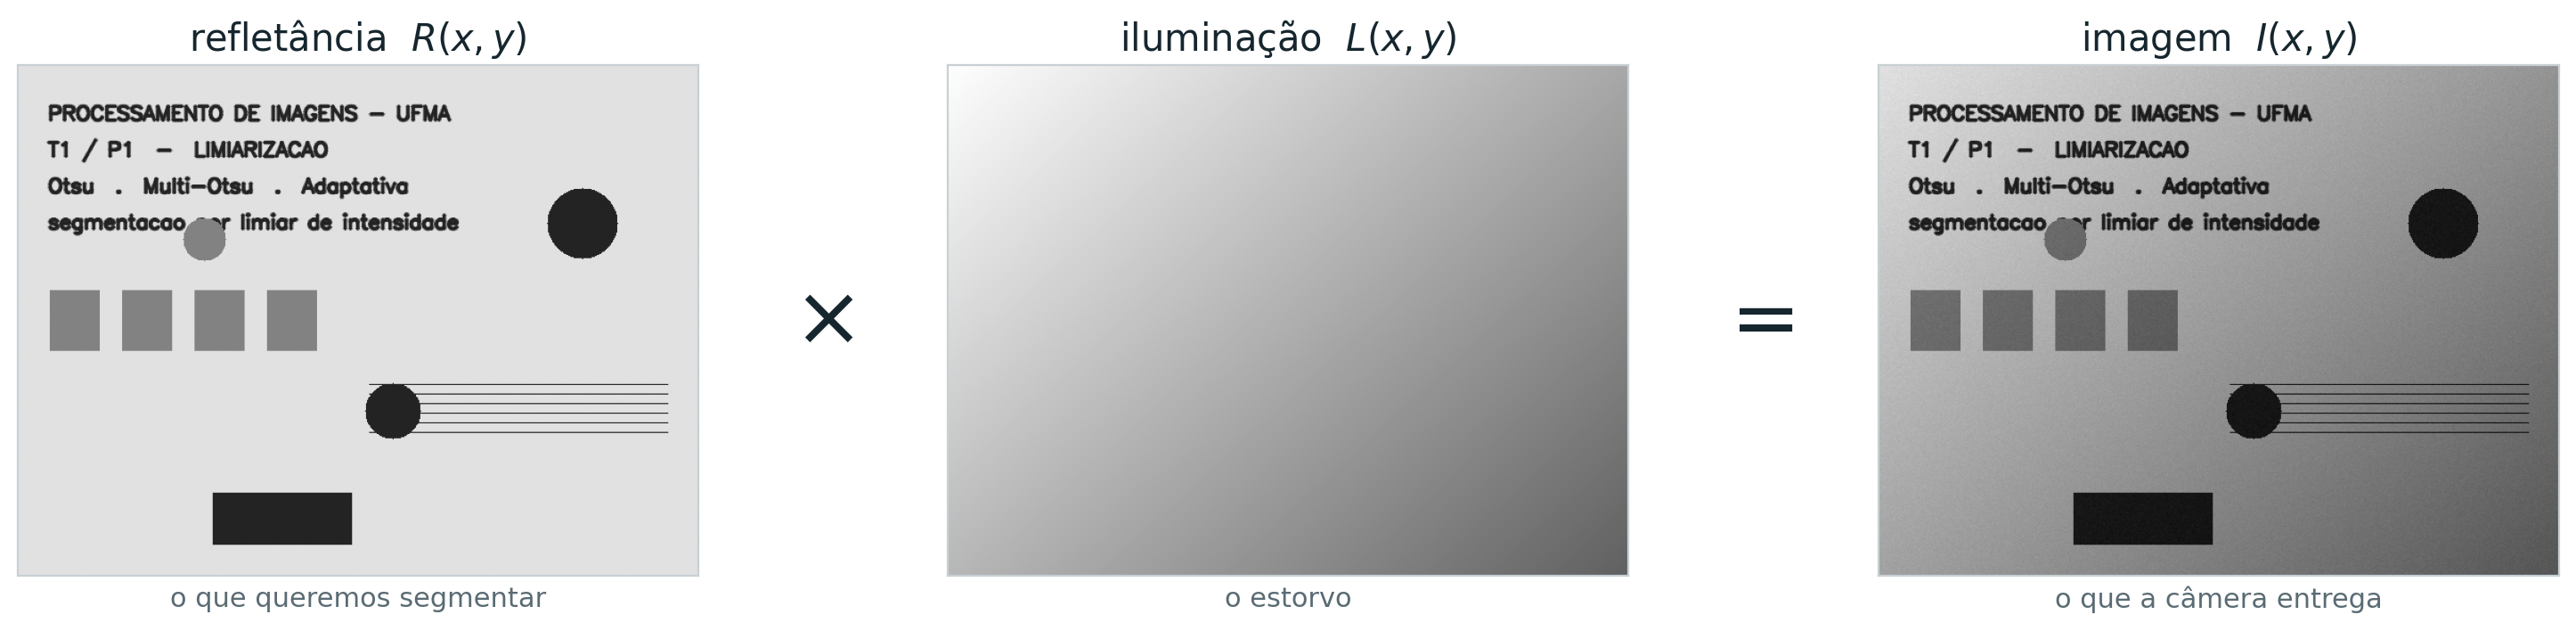
\includegraphics[width=\textwidth]{modelo_formacao}
  \end{center}

  \[
    I(x,y) = R(x,y)\cdot L(x,y) + n(x,y)
  \]

  \vspace{-.4em}
  Um limiar global só é válido se a iluminação $L$ for aproximadamente constante
  na imagem. Se a luz varia dentro da cena, o fundo de uma região escura fica
  mais escuro que o objeto de uma região clara.

\end{frame}

% =============================================================================
\begin{frame}{A mídia usada}

  \begin{center}
    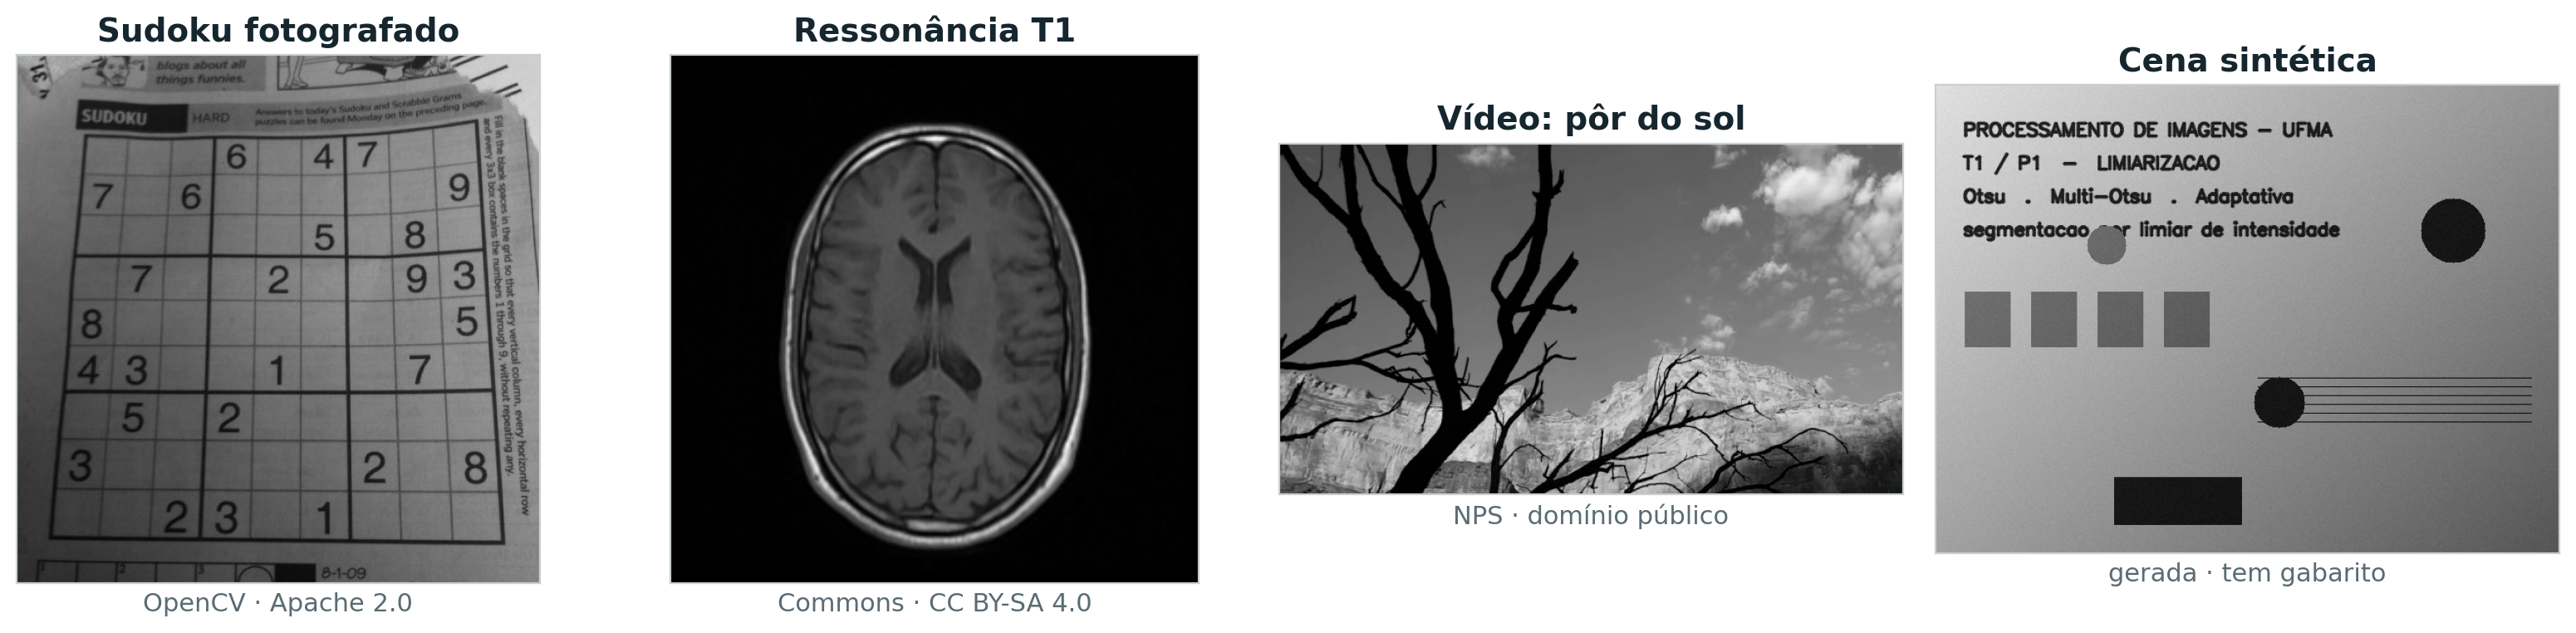
\includegraphics[width=\textwidth]{midia}
  \end{center}

  \vspace{-.2em}
  As três primeiras são reais e de licença livre. A quarta foi gerada por nós,
  e é a única com \textbf{gabarito}: sabemos a resposta certa em cada pixel.

  \vspace{.3em}
  \leg{Isso importa porque IoU e F1 comparam contra um gabarito. Em imagem real
  ninguém sabe a resposta pixel a pixel, então lá a comparação é visual e pelo
  comportamento do limiar.}

\end{frame}

% =============================================================================
\section{Otsu}

% -----------------------------------------------------------------------------
\begin{frame}{Método de Otsu (1979)}

  O histograma normalizado $p(i)$ é tratado como distribuição de probabilidade.
  Um limiar $t$ separa duas classes, com pesos $\omega_k$ e médias $\mu_k$.

  \vspace{.3em}
  \begin{columns}[T,onlytextwidth]
    \column{.47\textwidth}
      Variância dentro das classes:
      \[ \sigma_W^2(t)=\omega_0\sigma_0^2+\omega_1\sigma_1^2 \]
    \column{.47\textwidth}
      Variância entre as classes:
      \[ \sigma_B^2(t)=\omega_0\,\omega_1\,(\mu_0-\mu_1)^2 \]
  \end{columns}

  \vspace{.5em}
  Vale a identidade $\sigma_T^2 = \sigma_W^2(t) + \sigma_B^2(t)$, e $\sigma_T^2$
  não depende de $t$. Logo maximizar $\sigma_B^2$ equivale a minimizar
  $\sigma_W^2$, e o critério é

  \[ t^{*} = \arg\max_t \;\sigma_B^2(t) \]

  \vspace{-.2em}
  Custo $O(N)$, uma passada pela imagem: 0,16~ms por quadro de 640$\times$480.

\end{frame}

% -----------------------------------------------------------------------------
\begin{frame}{Otsu: histograma e critério}

  \begin{center}
    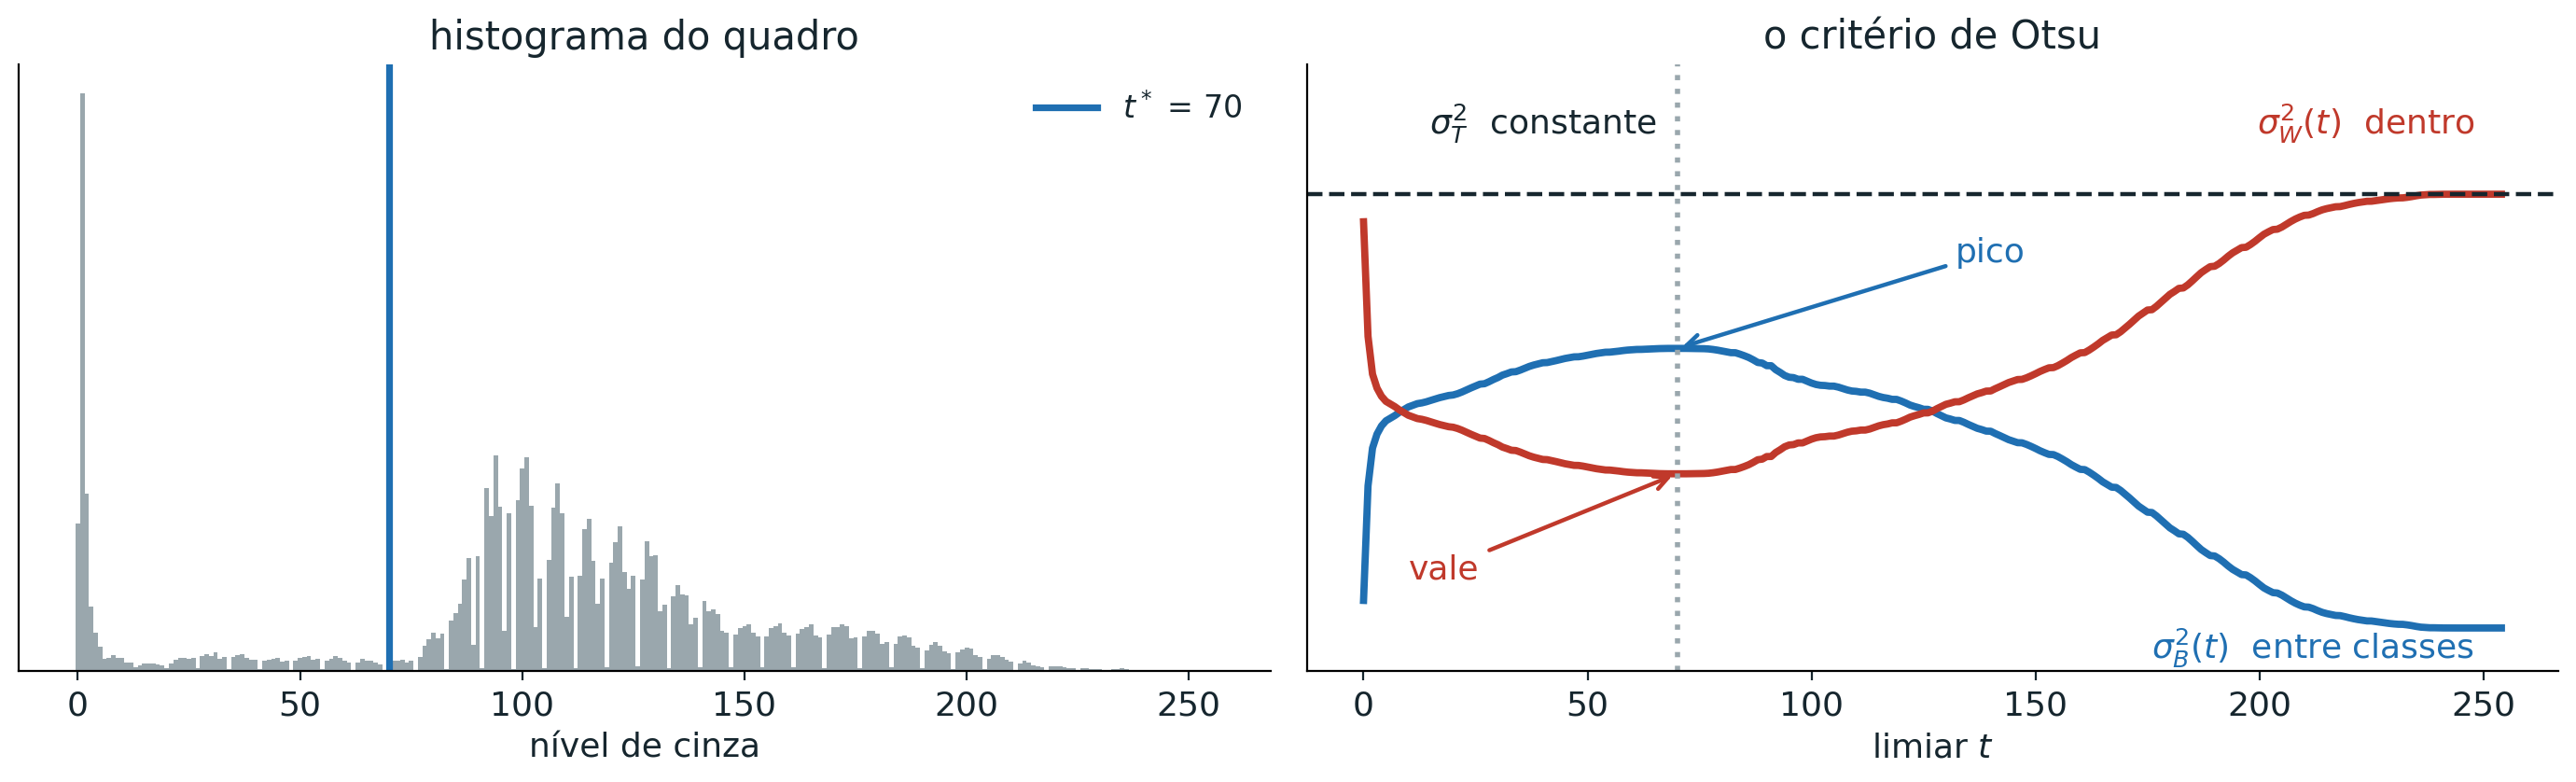
\includegraphics[width=\textwidth]{otsu_anatomia}
  \end{center}

  \leg{Sobre um quadro do vídeo. O pico da variância entre classes coincide com
  o vale da variância dentro das classes, e a soma das duas é constante. O
  limiar escolhido é o do pico.}

\end{frame}

% -----------------------------------------------------------------------------
\begin{frame}{Otsu no vídeo real}

  \begin{center}
    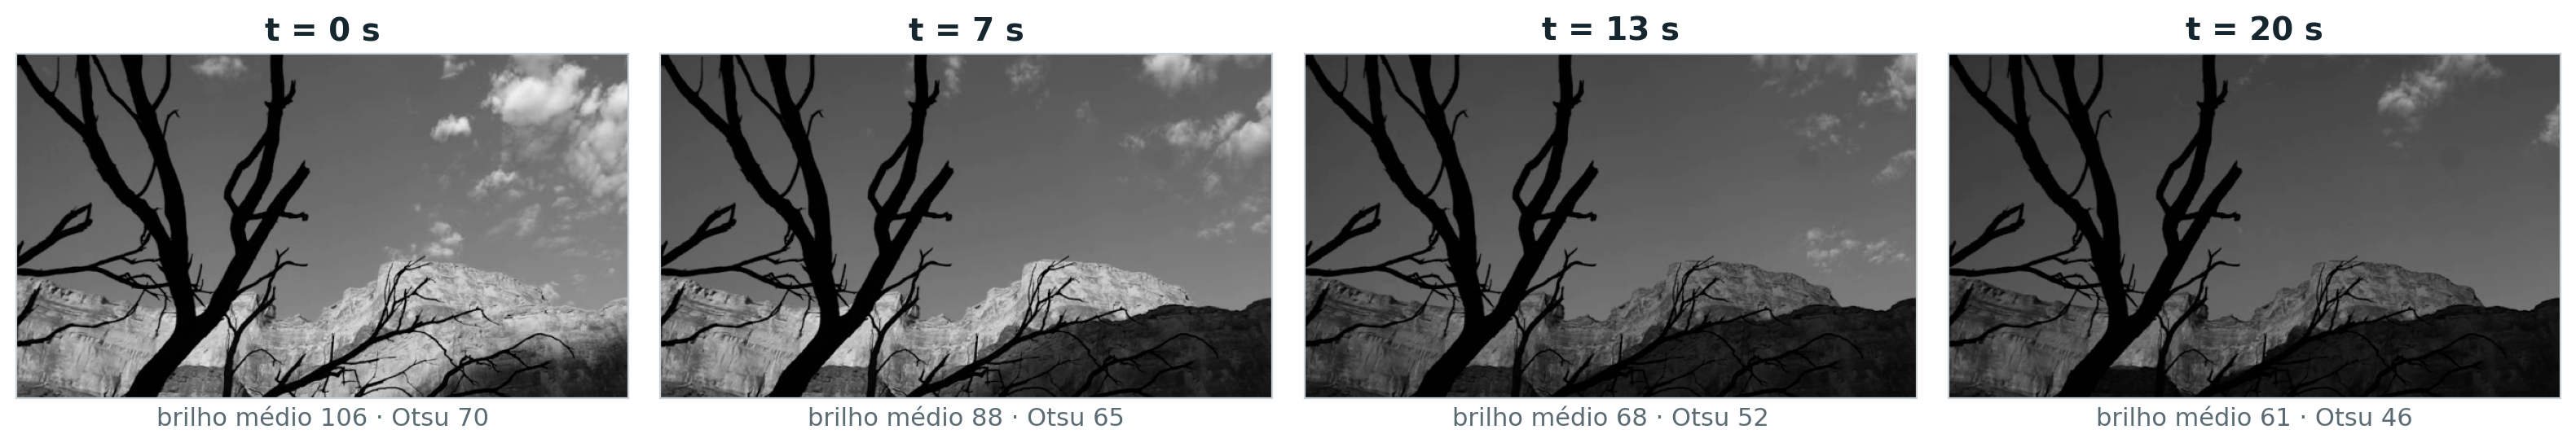
\includegraphics[width=\textwidth]{video_real_strip}
  \end{center}

  \vspace{-.2em}
  Ao longo dos 20~s o sol se põe: o brilho médio cai de 106 para 62. O Otsu
  recalcula o limiar a cada quadro e o desce sozinho de \textbf{70 para 46}.

  \vspace{.4em}
  Nenhum parâmetro foi ajustado entre um quadro e outro. É a mesma linha de
  código, lendo um histograma diferente.

\end{frame}

% =============================================================================
\section{Multi-Otsu}

% -----------------------------------------------------------------------------
\begin{frame}{Multi-Otsu}

  Muitas cenas têm mais de duas populações de cinza: documento com papel, tinta
  e sombra; ressonância com fundo, tecido e osso. Forçar duas classes funde duas
  populações distintas.

  \vspace{.4em}
  O critério é a extensão direta do de Otsu para $M$ classes e $M-1$ limiares:

  \[
    \sigma_B^2(t_1,\dots,t_{M-1}) = \sum_{k=0}^{M-1}\omega_k\,(\mu_k-\mu_T)^2
  \]

  \vspace{-.2em}
  A saída não é binária, e sim um mapa de rótulos (\texttt{np.digitize}).
  Para obter uma máscara binária é preciso decidir em qual limiar cortar, e essa
  decisão é do projetista.

\end{frame}

% -----------------------------------------------------------------------------
\begin{frame}{O custo da busca}

  \begin{columns}[c,onlytextwidth]
    \column{.44\textwidth}
      \footnotesize
      \begin{tabular}{@{}ccr@{}}
        \toprule
        $M$ & limiares & combinações \\
        \midrule
        2 & 1 & 255 \\
        3 & 2 & 32\,385 \\
        4 & 3 & 2\,731\,135 \\
        5 & 4 & 172\,061\,505 \\
        \bottomrule
      \end{tabular}

      \vspace{.8em}
      \normalsize
      A busca exaustiva testa $\binom{L-1}{M-1}$ combinações e se torna
      inviável a partir de $M=5$.

    \column{.52\textwidth}
      Solução em duas partes:

      \begin{itemize}
        \item tabelas de momentos (Liao, Chen \& Chung, 2001), com
          $H(u,v) = S(u,v)^2/P(u,v)$;
        \item programação dinâmica sobre essas tabelas,
          $D[m][v]=\max_{u<v}\bigl(D[m{-}1][u]+H(u{+}1,v)\bigr)$.
      \end{itemize}

      \vspace{.4em}
      O custo cai para $O(M L^2)$, cerca de 1,3~ms para $M=3$.
  \end{columns}

\end{frame}

% -----------------------------------------------------------------------------
\begin{frame}{Multi-Otsu na ressonância}

  \begin{center}
    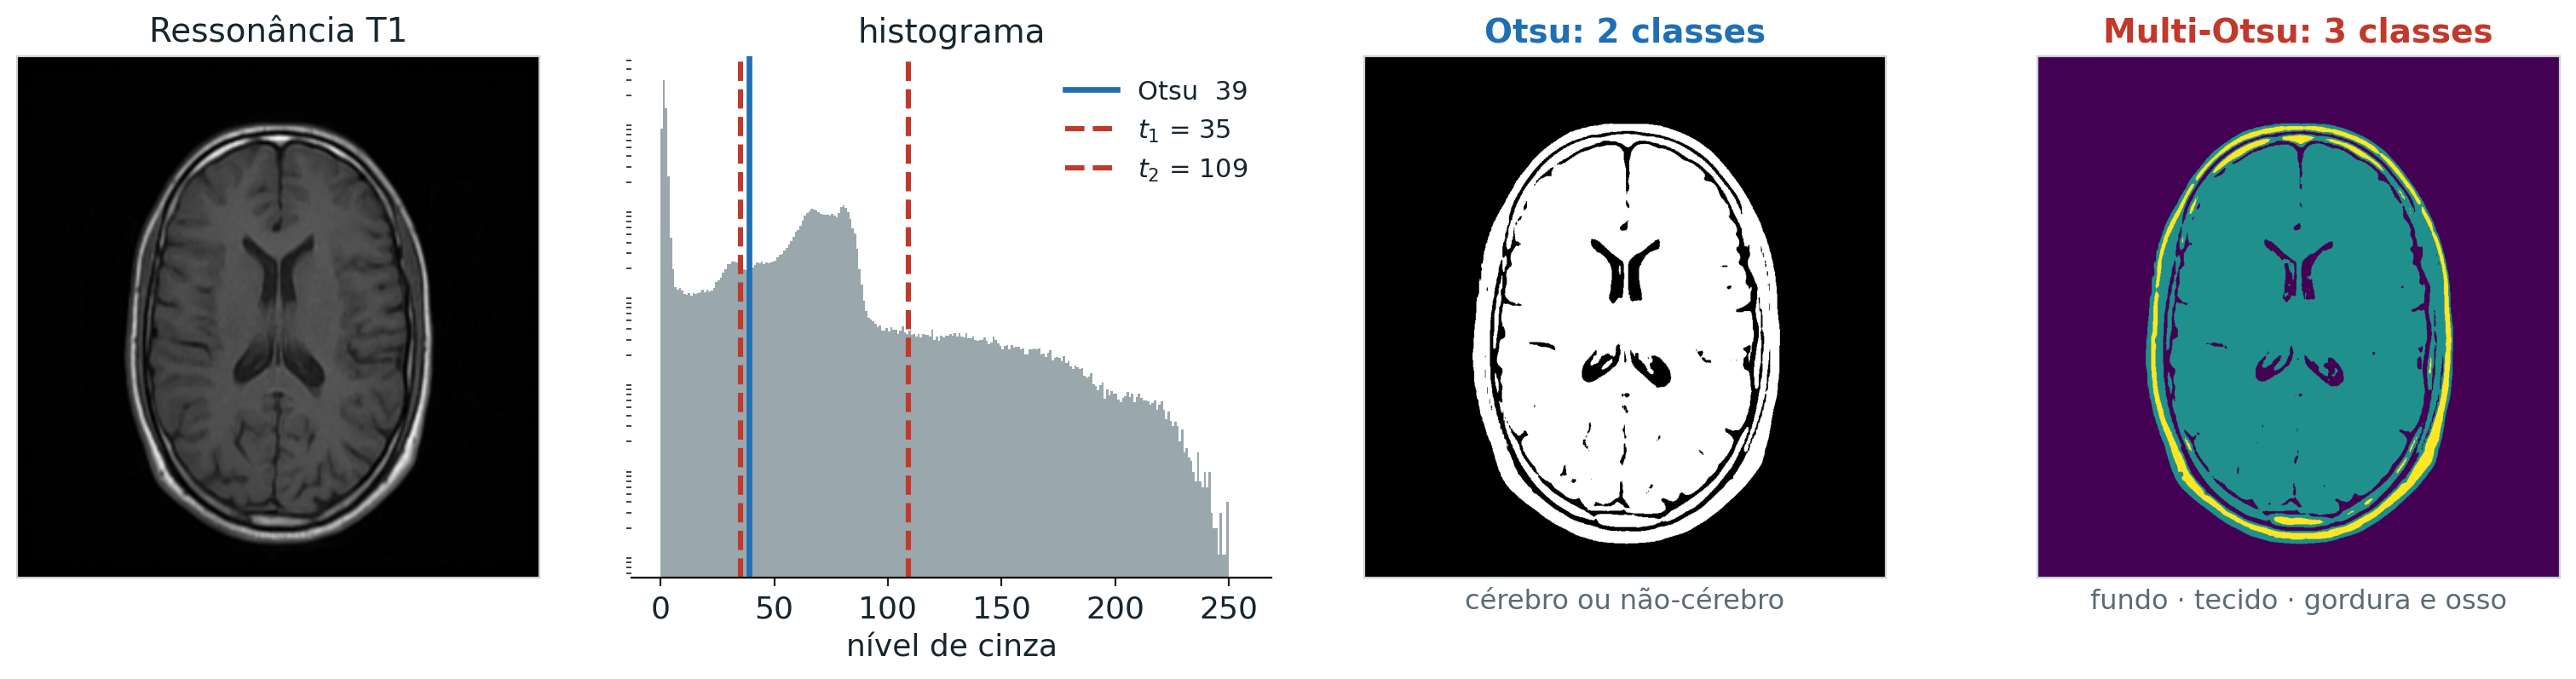
\includegraphics[width=\textwidth]{multiotsu_mri}
  \end{center}

  \vspace{-.3em}
  Com duas classes só dá para responder "cérebro ou não-cérebro". Com três, a
  gordura e o osso do crânio saem separados do tecido cerebral.

  \vspace{.3em}
  \leg{Aumentar $M$ sempre aumenta $\sigma_B^2$, então $M$ não pode ser
  escolhido maximizando o próprio critério. É um hiperparâmetro.}

\end{frame}

% =============================================================================
\section{Limiarização adaptativa}

% -----------------------------------------------------------------------------
\begin{frame}{Limiarização adaptativa}

  \begin{center}
    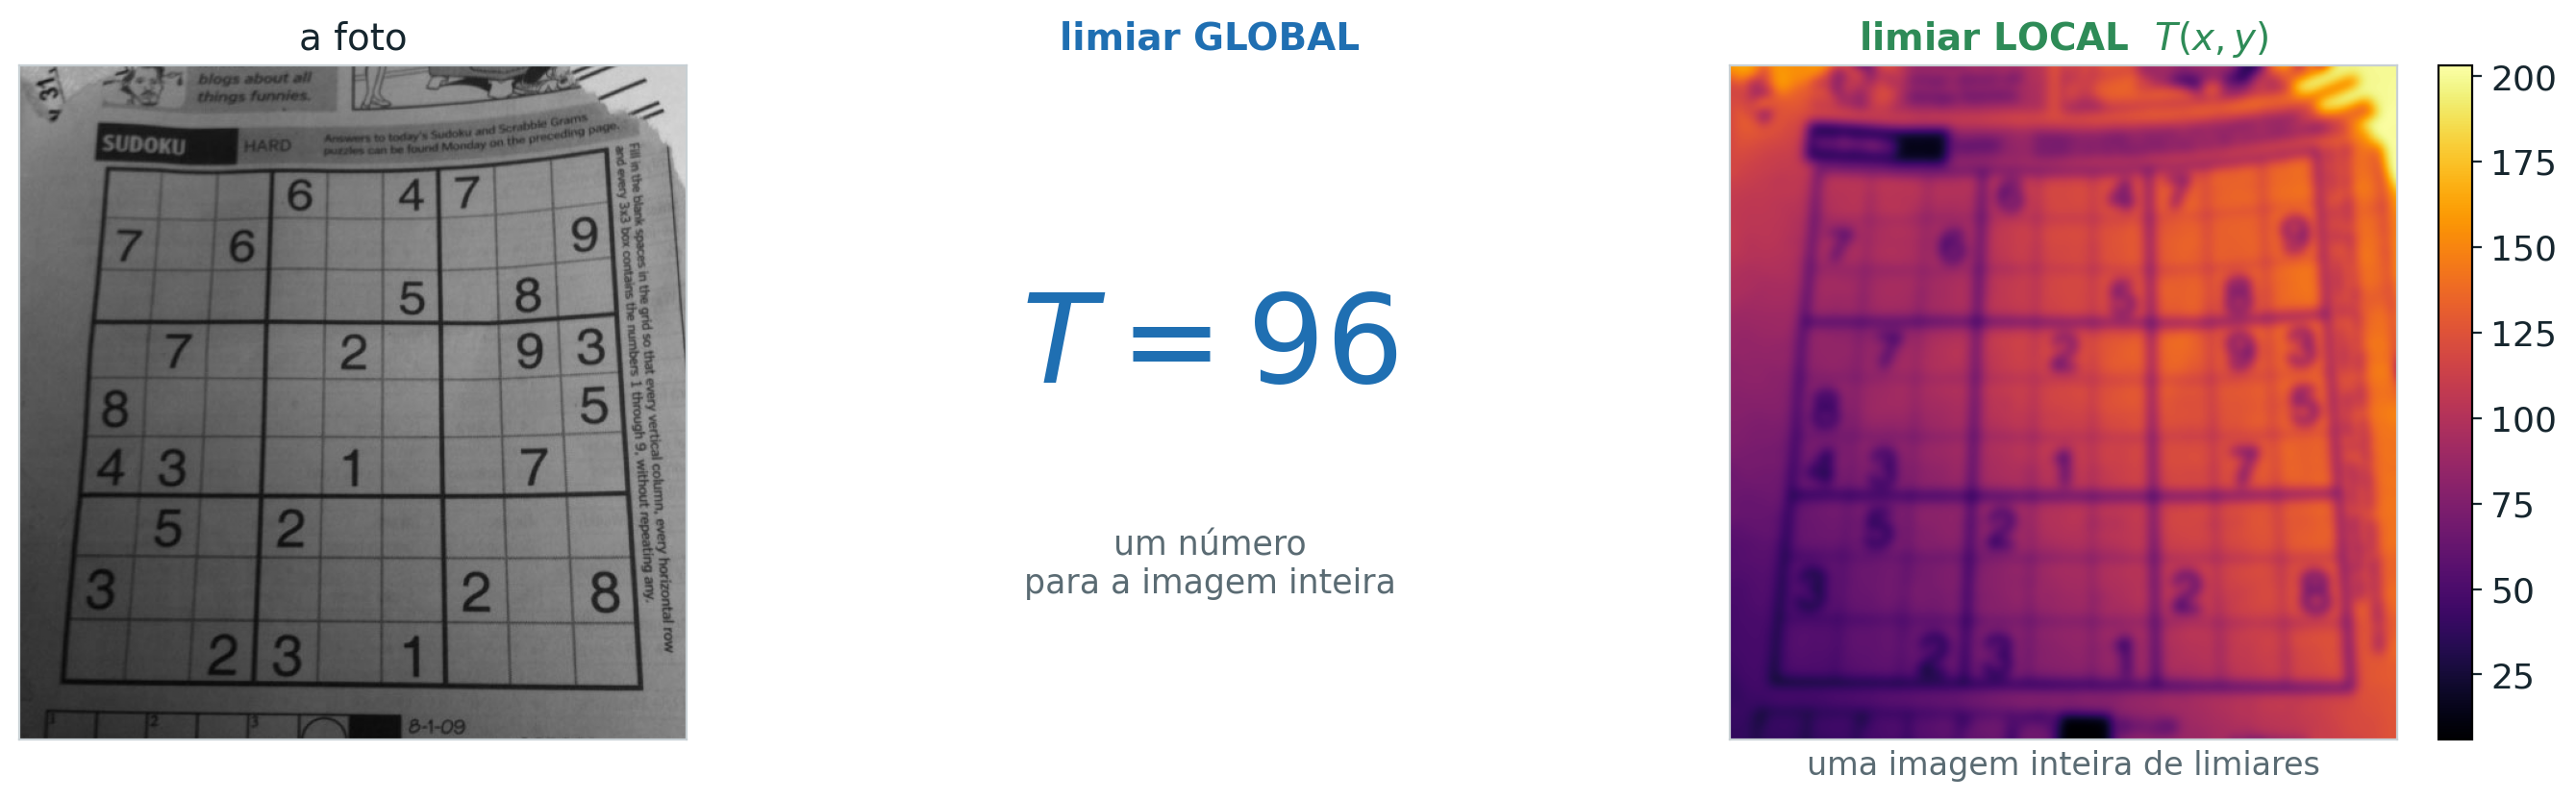
\includegraphics[width=.94\textwidth]{limiar_global_vs_local}
  \end{center}

  \vspace{-.3em}
  O limiar deixa de ser um número e passa a ser uma imagem, calculada a partir
  da vizinhança $b \times b$ de cada pixel: \;$T(x,y) = m(x,y) - C$.

  \vspace{.2em}
  \leg{Repare que o mapa $T(x,y)$ é praticamente uma estimativa da iluminação da
  cena. É isso que permite acompanhar a sombra.}

\end{frame}

% -----------------------------------------------------------------------------
\begin{frame}{Os dois parâmetros}

  \begin{center}
    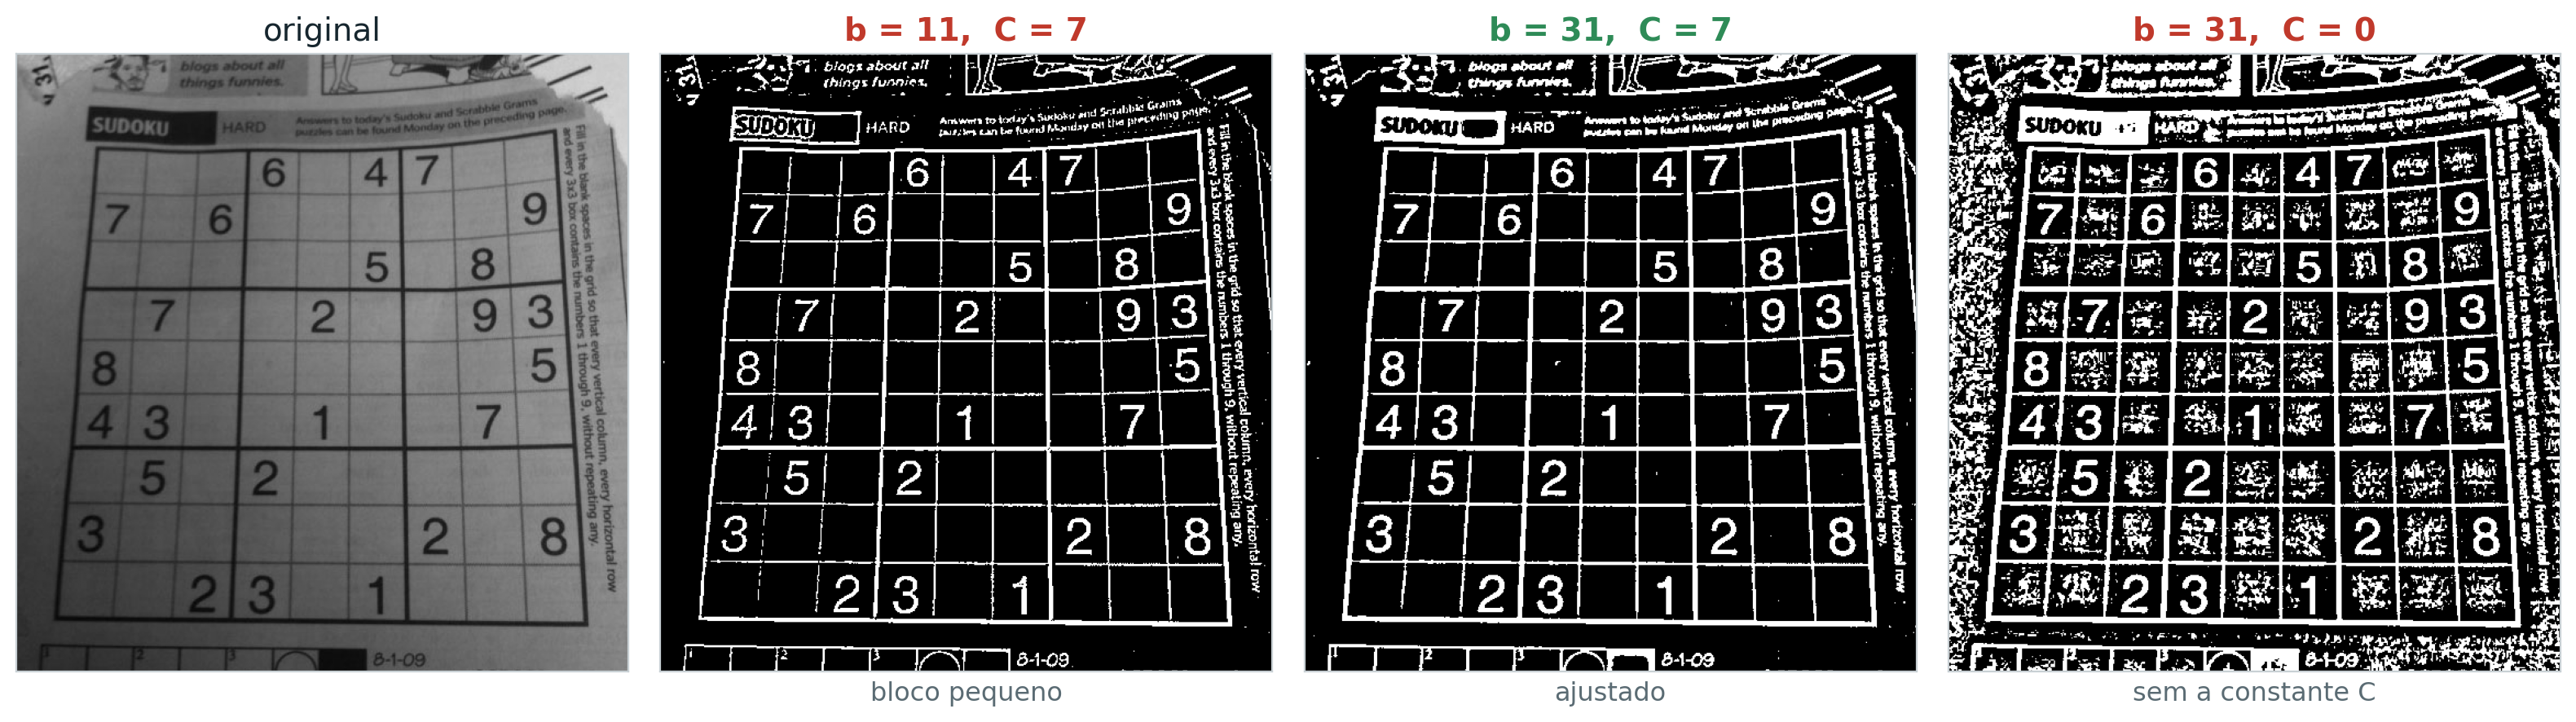
\includegraphics[width=\textwidth]{parametros}
  \end{center}

  \vspace{-.4em}
  \begin{columns}[T,onlytextwidth]
    \column{.47\textwidth}
      \textbf{Bloco $b$.} Maior que o traço a detectar, menor que a escala em
      que a luz varia. Pequeno demais, só a borda sobrevive.
    \column{.47\textwidth}
      \textbf{Constante $C$.} Em região lisa $I \approx m$, e sem $C$ o
      resultado é o sinal do ruído. $C$ cria a margem.
  \end{columns}

\end{frame}

% -----------------------------------------------------------------------------
\begin{frame}{A demonstração}

  \begin{center}
    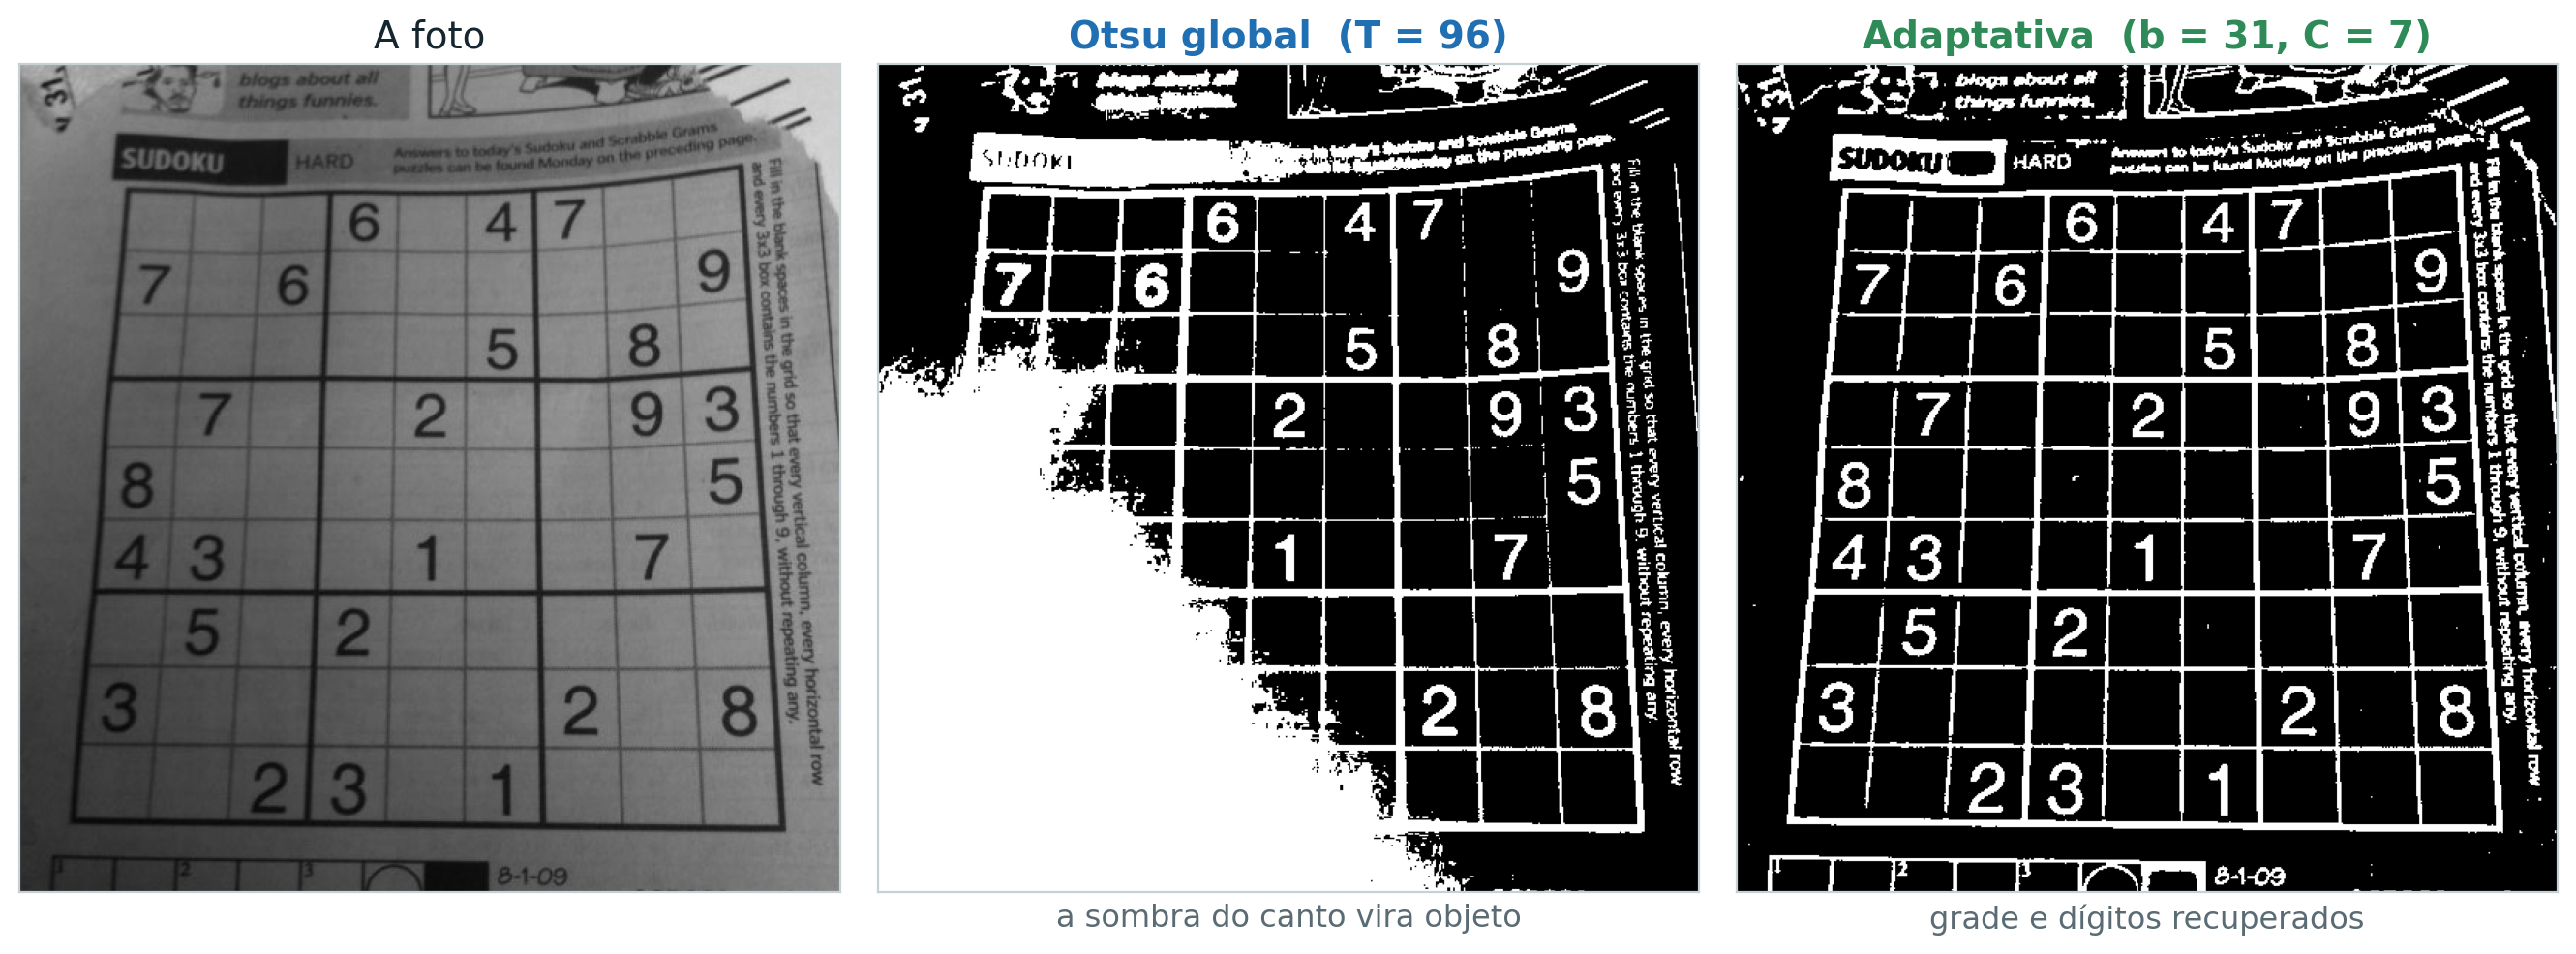
\includegraphics[width=\textwidth]{sudoku}
  \end{center}

  \vspace{-.4em}
  A foto é a do próprio tutorial do OpenCV, com o canto superior esquerdo na
  sombra. O Otsu escolhe o melhor $T$ possível e mesmo assim perde a região
  inteira: a sombra é mais escura que a tinta do lado iluminado.

\end{frame}

% =============================================================================
\section{Comparação}

% -----------------------------------------------------------------------------
\begin{frame}{O limiar ao longo do vídeo}

  \vspace{-.3em}
  \begin{center}
    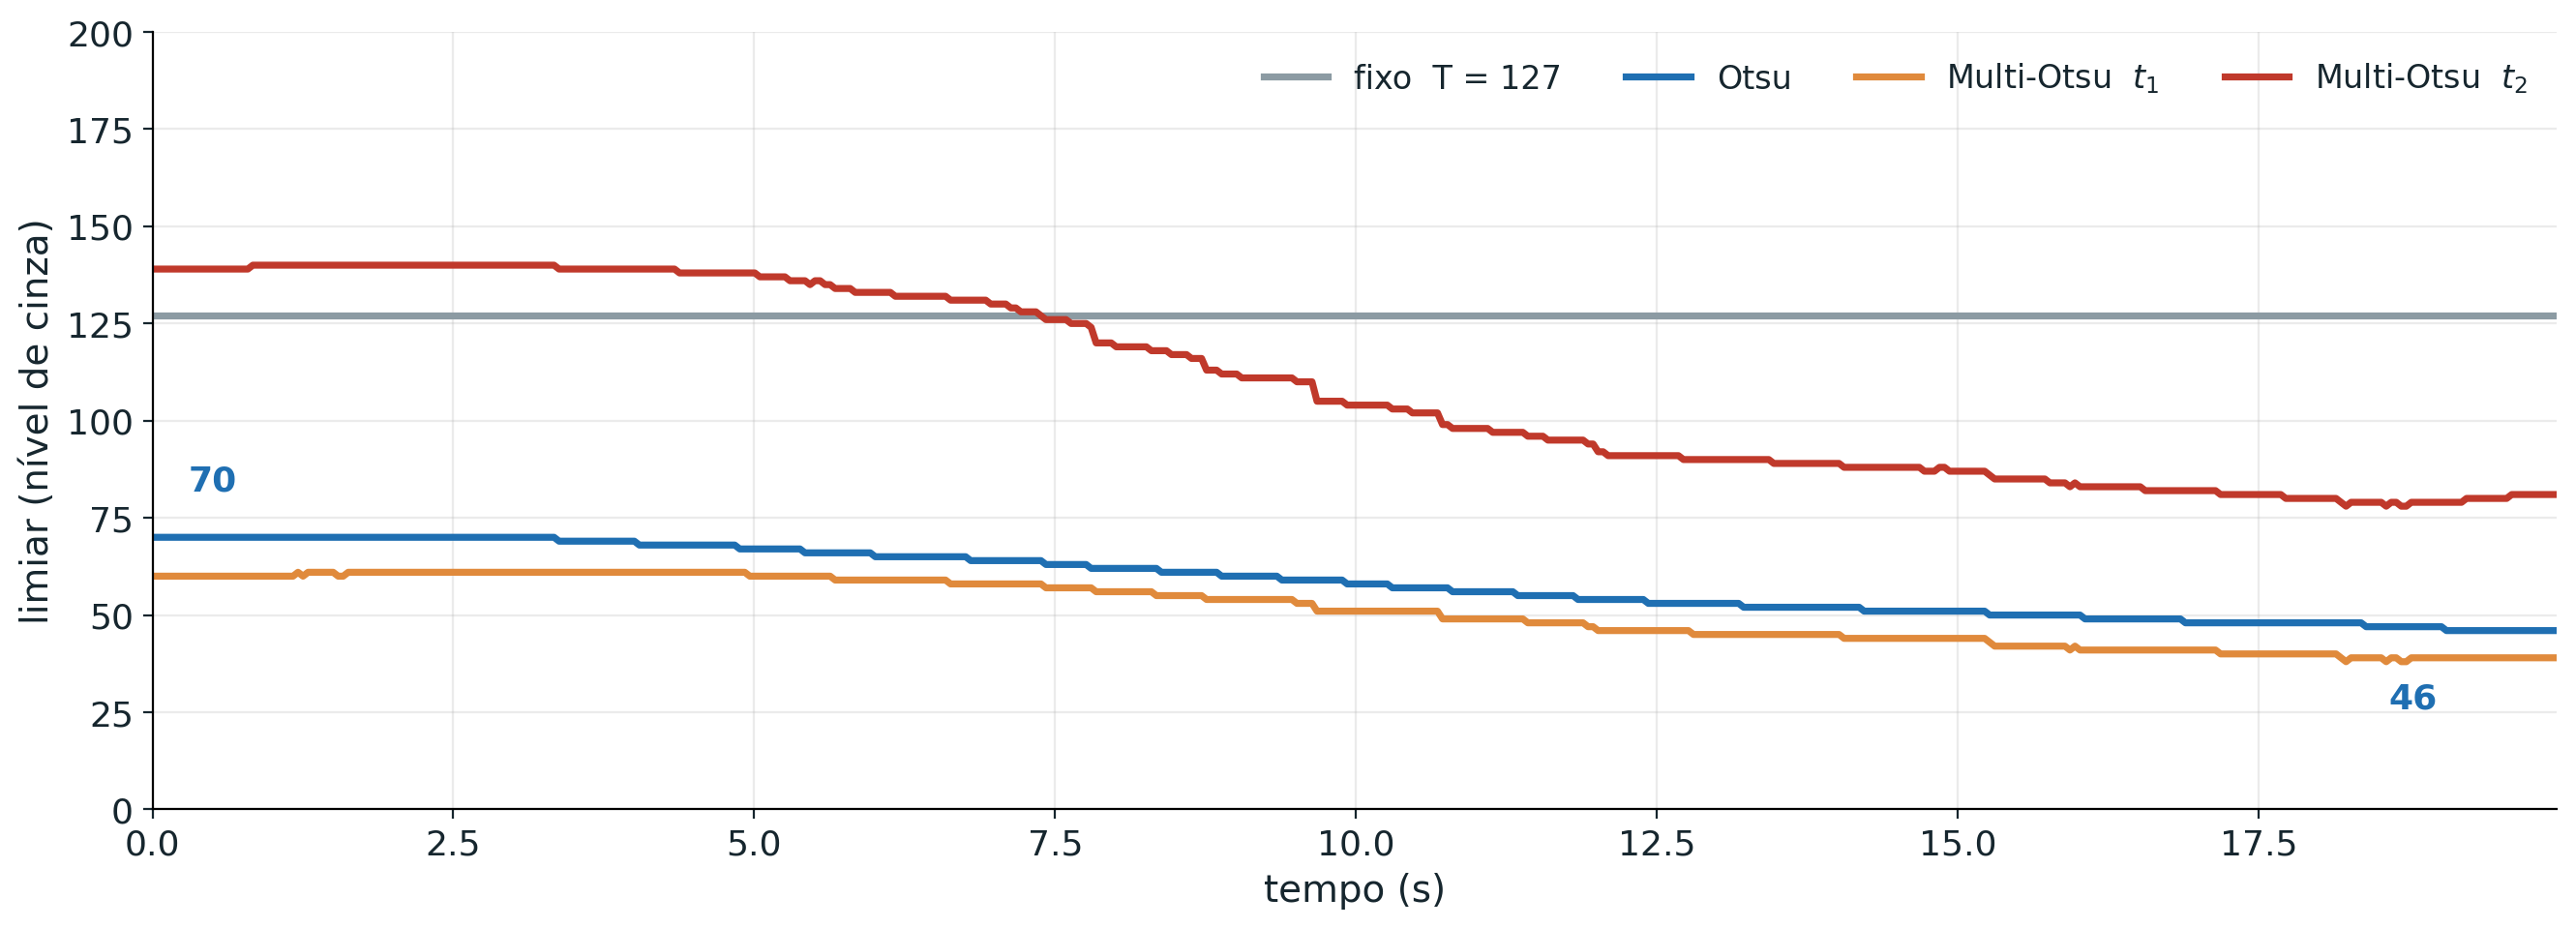
\includegraphics[width=.92\textwidth]{limiar_canyon}
  \end{center}

  \vspace{-.6em}
  \leg{Os métodos automáticos acompanham o pôr do sol. O limiar fixo, em cinza,
  não se move: ele começa classificando 67\,\% da imagem como objeto e termina
  com \textbf{99,6\,\%}, ou seja, praticamente tudo.}

\end{frame}

% -----------------------------------------------------------------------------
\begin{frame}{Para medir, é preciso gabarito}

  Em imagem real não há resposta certa pixel a pixel. Por isso geramos também
  uma cena sintética de 20~s, com gabarito em cada quadro e quatro fases que
  isolam um fator cada.

  \vspace{.6em}
  \begin{center}
  \small
  \begin{tabular}{@{}lccccc@{}}
    \toprule
    Método & \textbf{1} uniforme & \textbf{2} sombra & \textbf{3} escurece
           & \textbf{4} ruído & Global \\
    \midrule
    Limiar fixo $T=127$      & 0,657 & 0,140 & 0,636 & 0,634 & 0,516 \\
    Otsu                     & 0,944 & 0,139 & 0,943 & \textbf{0,834} & 0,715 \\
    Multi-Otsu $t_1$         & 0,592 & 0,731 & 0,600 & 0,639 & 0,641 \\
    Multi-Otsu $t_2$         & 0,966 & 0,138 & \textbf{0,965} & 0,626 & 0,674 \\
    Adaptativa               & \textbf{0,971} & \textbf{0,956} & 0,950 & 0,575 & \textbf{0,863} \\
    \bottomrule
  \end{tabular}
  \end{center}

  \vspace{.4em}
  \leg{Na fase 2 a luz varia \emph{dentro} do quadro e os globais colapsam. Na
  fase 4 a ordem se inverte.}

\end{frame}

% -----------------------------------------------------------------------------
\begin{frame}{Onde cada método erra}

  \vspace{-.3em}
  \begin{center}
    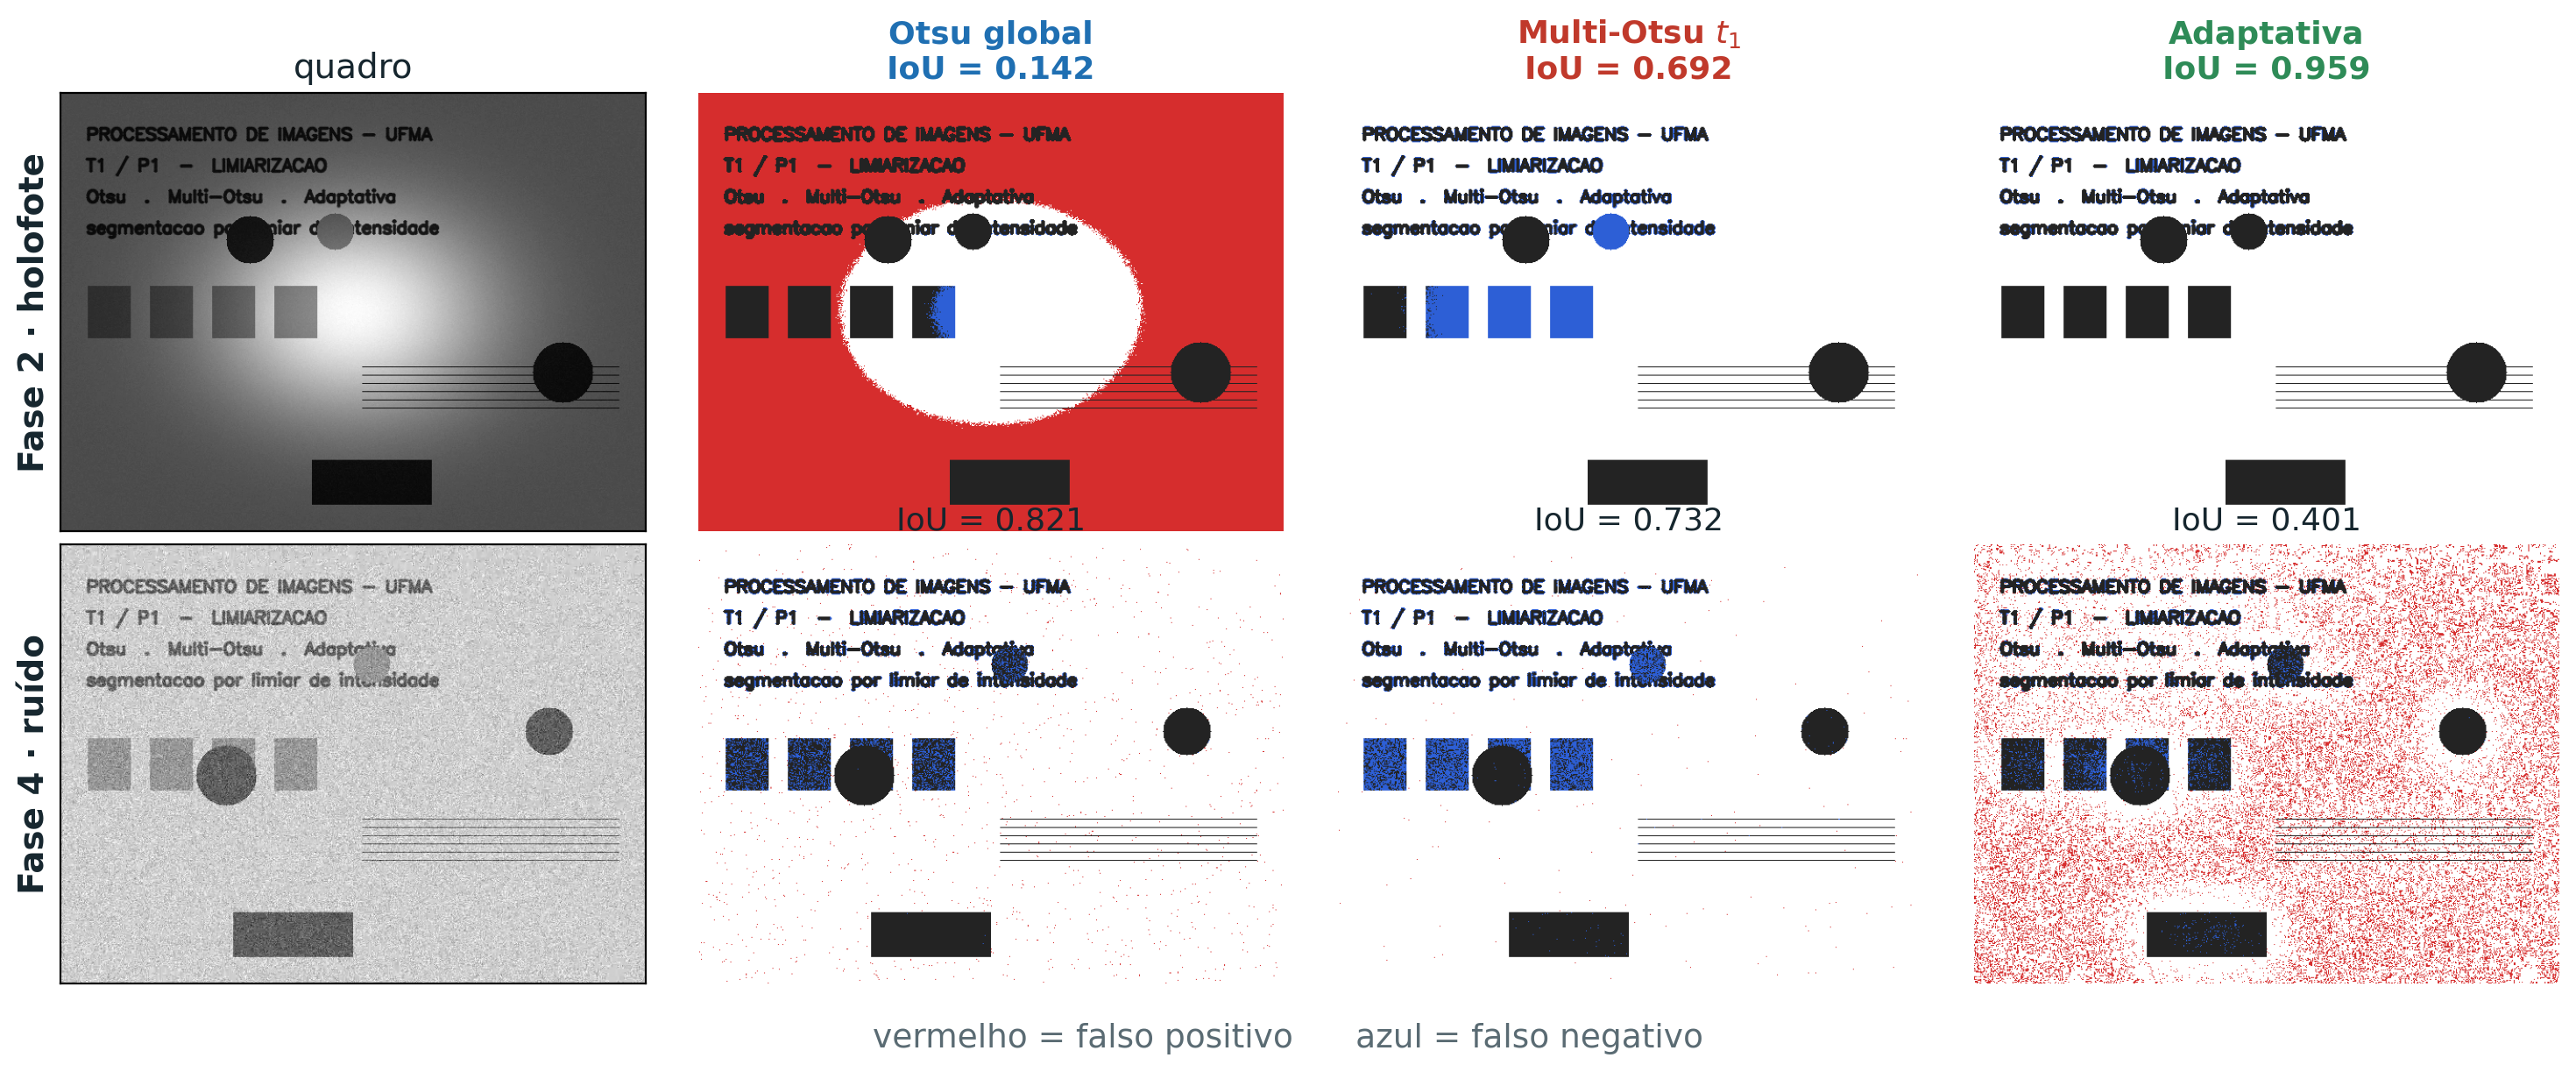
\includegraphics[width=.90\textwidth]{erros_slide}
  \end{center}

  \vspace{-.5em}
  \leg{Com sombra, o Otsu classifica como objeto todo o fundo escurecido. Com
  ruído, é a adaptativa que fica coberta de falsos positivos. A ordem dos
  métodos se inverte entre as duas linhas.}

\end{frame}

% =============================================================================
\begin{frame}{Conclusão}

  \begin{itemize}
    \item O limiar global falha com variação \textbf{espacial} de iluminação,
      não com variação temporal. No vídeo real a cena escurece por completo e o
      Otsu acompanha sem perder qualidade; na cena com sombra ele vai de 0,944
      para 0,139.

    \item A limiarização adaptativa troca robustez à iluminação por fragilidade
      ao ruído. As duas coisas vêm da mesma causa: ela decide a partir de poucos
      pixels.

    \item Nenhum método venceu todas as situações. A escolha depende de qual
      hipótese a cena satisfaz, não de qual técnica é melhor.
  \end{itemize}

  \vspace{.6em}
  \leg{Limitações: a parte quantitativa usa cena sintética, porque é o que
  permite ter gabarito; usamos um único ajuste de parâmetros por método; e não
  houve pós-processamento morfológico, que mudaria o resultado da fase de ruído.}

\end{frame}

% -----------------------------------------------------------------------------
\begin{frame}[standout]
  Obrigado
\end{frame}

% -----------------------------------------------------------------------------
\begin{frame}{Créditos e referências}

  \footnotesize
  \textbf{Mídia}

  \begin{itemize}
    \item Foto do sudoku: projeto \textbf{OpenCV}, \texttt{samples/data/sudoku.png},
      licença Apache 2.0. É a imagem do tutorial \emph{Image Thresholding}.
    \item Ressonância: \textbf{MRI Brain T1 Axial (12)}, autor 511KeV,
      Wikimedia Commons, \textbf{CC BY-SA 4.0}.
    \item Vídeo: \emph{Colorado River Time-lapse and Sunset}, Grand Canyon
      National Park / \textbf{National Park Service}, domínio público, via
      Wikimedia Commons.
    \item Cena sintética: gerada pelo código deste trabalho.
  \end{itemize}

  \vspace{.1em}
  \textbf{Bibliografia}

  \scriptsize
  \begin{itemize}
    \item Otsu, N. \emph{A Threshold Selection Method from Gray-Level
      Histograms}. IEEE Trans. SMC, 9(1):62--66, 1979.
    \item Liao, Chen \& Chung. \emph{A Fast Algorithm for Multilevel
      Thresholding}. J. Inf. Sci. Eng., 17:713--727, 2001.
    \item Bradley \& Roth. \emph{Adaptive Thresholding using the Integral
      Image}. J. Graphics Tools, 12(2):13--21, 2007.
    \item Gonzalez \& Woods. \emph{Digital Image Processing}, cap. 10.
      Tutoriais: scikit-image \texttt{plot\_thresholding} e
      \texttt{plot\_multiotsu}; OpenCV \texttt{py\_thresholding}.
  \end{itemize}

\end{frame}

\end{document}
